\section{A Closed-form Solution}

In nature, most organic models ubiquitously contain cylindrical parts \cite{Zhou:2015:GCD}, e.g., arms, legs, etc. Moreover, a cylindrical part can be well represented by its corresponding {\color{red}curved} skeleton. Based on this property, a chunk of a mesh model can be fabricated free of support {if all the arcs of its corresponding skeleton arc subtend to a printing direction by an angle of no large than $\theta$ (Figure \ref{fig:spike}).} Hence, our problem becomes partitioning a given 1{D} skeleton graph into a set of subgraphs such that each subgraph merits the desirable support-free property. In the remainder of the paper, by model we mean an organic mesh model of natural life form or articulated figures preserving nice topology features of real lives.

\begin{figure}[t!]
  \centering
  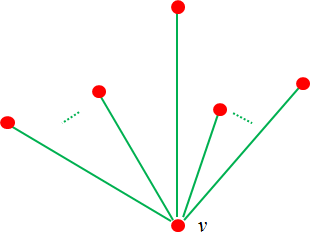
\includegraphics[width=\linewidth]{figs/fork.png}
  \caption{\label{fig:fork}%
  A segment (a) of a skeleton corresponds to a fork (b) originated from a node. (c) A subgraph which can be support-free printed.}
\end{figure}

\textbf{Choice of skeleton.} Compared to natural skeletons, the medial axis can describe the topology of a mesh model more precisely \cite{ZhangXWYTW15}. However, a medial axis of a 3D mesh model is a 2D surface which cannot be conveniently applied to describe the critical topology changes of the model. Additionally, the medial axis consists of intersecting pieces of planes and conic surfaces, presenting significant complications to algorithms that attempt to construct 3D medial axes.
Reeb graph provides a possible choice for the curve skeleton. During the generation process of any Reeb graph, the slicing direction and the position of the representative node on each slice (a connected region) seriously influence the choice of critical points. Moreover, the determination of suitable slicing direction and representative nodes is an intractable problem. {\color{red}There are quite a few methods that generate curve skeletons from a 3D model. For example, medial surface based method which contracts the medial axis surface of the model; the generalized field method which by trace curves seeded at critical points along high-divergence directions \cite{rumpf2002continuous}; and contraction methods which shrink the mesh into curves \cite{AuTCCL08,tagliasacchi20163d}. It is hard to analytically compare the properties of the curve skeleton due to the lack of a unanimously accepted formal definition of skeleton. For a complete survey of these methods, the readers are referred to the survey paper \cite{tagliasacchi2009curve}. To carry on our methodology of partitioning the model based on curve skeletons,} we resort to the Laplacian skeleton proposed by \cite{AuTCCL08} which is extracted by shrinking the mesh model using Laplacian smoothing, such a curve skeleton provides an excellent choice for reasonably describing the geometrical and topological variations of any 3{D} model. The Laplacian Skeleton represents the models very well if the following two conditions are met: {(1) each critical topological feature of the model is captured by the skeleton; (2) the skeleton is dense enough to capture the geometric variations of the original shape.

\begin{figure}[b!]
  \centering
  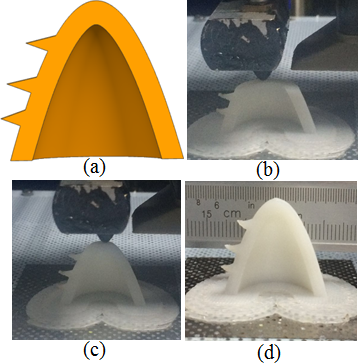
\includegraphics[width=\linewidth]{figs/spike.png}
  \caption{\label{fig:spike}%
           Support-free printing of a model with some spikes on it: the length of the spikes is $4 mm$, the overhang angle is 15 degrees, the model is fabricated by a Zortrax M200 3D printer.}
\end{figure}

For condition (1), we use the $1D$ Laplacian skeleton provided by the authors of \cite{AuTCCL08}, which has been shown to be capable of segmenting complicated models in a nice way. For condition (2), the density of the skeleton, one can always add arcs (line segments) into the skeleton and obtain a finer representation of a smaller strip of the mesh model. In special cases, a portion of the mesh is not represented properly by a Laplacian Skeleton arc if it is a tinny detail that have been shrunk into a point during just a few iterations of the Laplacian smoothing process. We find that these details can usually be printed out in a support-free manner if the overhang angle is not that small (e.g., larger than 10 degrees) with respect to the building platform, and that the overhang length is within a safe distance (e.g., 1-5mm) when a nozzle jumps from one point to another. See Figure \ref{fig:spike} for an illustration. We remark that this distance is long enough to address most cases when small details are not captured by a skeleton arc: it can also be printed out by any prevailing desktop 3D printer in a support-free manner due to the cohesive and elastic forces that are inherent to the plastic material itself. }




%Figure \ref{fig:ex1} shows an example of the Laplacian skeleton.

%\begin{figure}[tbp]
%  \centering
% \mbox{} \hfill
%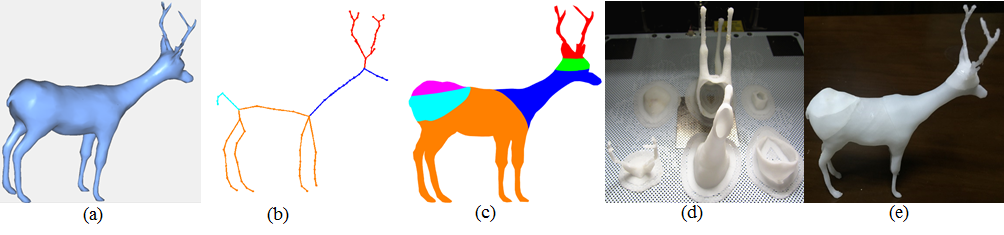
\includegraphics[width=0.4\textwidth]{figs/tree_with_skeleton.png}
%\caption{\label{fig:ex1}%
%        An illustration of a 3D mesh model and its 1D Laplacian skeleton. }
%\end{figure}



\textbf{Problem Statement.} Our goal is hence to decompose the Laplacian skeleton of the model into {{a proper number of support-free subgraphs leading to a partition of the model into the least number of printable parts free of support structures and seams on the final assembled model.}} In addition, since support structures result in bumpy supported areas, support-free fabrication also means a nice preservation of the surface quality of the parts. Further, a minimization of the number of cuts and the total cutting length means a minimum amount of seams and their lengths on the assembled model. Therefore, we focus on these two problems in this paper.

Finding a decomposition of the skeleton into the least pieces of support free subgraphs is a non-trivial task. As a simple example, {{suppose for simplicity that the least number of cuts on the skeleton corresponds to the least number of cuts on the mesh model}}, refer to Figure \ref{fig:fork}, consider a Laplacian skeleton that is a fork with $n$ arcs sharing a common origin; consider partitioning the fork into the least number of sub-forks such that each sub-fork can be packed into a cone of angle $2\theta$ in order to make the sub-fork support-free when fabricated in a given direction, where $\theta$ is defined based on the printing experiments as a safe angle allowing support-free fabrication.

\emph{\textbf{Theorem 1}: Partitioning a graph into the least number of support-free subgraphs is NP-hard.}

\emph{Proof}:
We shall complete the proof by transforming an instance of a known $NP$ hard problem into our problem in polynomial time.
First we need to show that our problem is in $NP$: The certificate is a set of arc-disjoint and rooted subgraphs partition of the input graph (skeleton), a certifier checks in polynomial time (i.e., $O(n^2)$) that the number of subgraphs is at most the given bound $K$, and that the rooted subgraphs satisfy the angle constraint of $2\theta$.
We shall reduce the Clique Cover problem to the skeleton partition problem, where the Clique Cover problem is covering a graph with the least number of cliques (complete graphs), which has been shown to be $NP$-hard \cite{karp1972reducibility}. We now show that Clique Cover $ \leq p$ Skeleton Partition (i.e., Clique Cover is polynomial-time reducible to Skeleton Partition). {It suffices to show that there exists an instance of Skeleton Partition problem which is $NP$-hard.} Let us consider the following instance of Clique Cover: an arbitrary planar $G(V, E)$ such that $|V| = n$ and each pair of nodes ($v_i$, $v_j$) is connected by an arc if $|v_iv_j|$ is no larger than a given bound $D$. We construct a skeleton $S$ of $n$ arcs rooted at a common node (a fork) as follows: select any triplet of nodes {$v_i$, $v_j$, $v_k$} from $G$ and construct a triplet of unit arcs $\{e_i, e_j, e_k\}$ in $S$, the angle between each pair of arcs $\{e_i, e_j\}$, denoted as $A(e_i, e_j)$, is defined as $A(e_i, e_j) = 2\theta|v_iv_j|/D$. See Figure \ref{fig:fork}, given this triplet of arcs as the basis (three distinct vectors in 3{D} space), we can construct each of the remaining arcs of $S$, denoted as $e_x$, which represents a node $v_x$ in $G$: the relative position of $e_x$ with respect to each element of $\{e_i, e_j, e_k\}$ is defined as the distance from $v_x$ to each element of $\{v_i, v_j, v_k\}$. This transformation takes $O(n^2)$ time.

%Youyi: please add in the following ref. [Karp] Karp, Richard, "Reducibility Among Combinatorial Problems", in Miller, R. E.; Thatcher, J. W., Proceedings of a Symposium on the Complexity of Computer Computations, Plenum Press, pp. 85�C103, 1972.



Now we claim that there is a clique cover in $G$ of size $K$ if and only if there is a skeleton partition of $S$ into $K$ support-free subgraphs (the angle between each pair of arcs is no larger than $2\theta$).
For if there is clique cover in $G$ of size $K$, then each clique in $G$ corresponds to a rooted subgraph of $S$ that satisfies the angle constraint. Conversely, if $S$ is partitioned into $K$ support-free subgraphs, then every pair of arcs in each subgraph satisfy the angle constraint, by the mapping relation, their corresponding nodes in $G$ form a clique. This completes the proof. \qed

This tells the difficulty of solving the problem of partitioning a 3D model into the least number of support free pieces. In the following, we showcase the problem into different scenarios and show that there exists polynomial solutions when the graph satisfies certain conditions.

\textbf{Tree case.} If the topology of the skeleton $S$ is a tree such that the degree of each node is bounded by a constant $d$, and the least number of support-free subgraphs is smaller than a constant $c$, we show that the problem of partitioning $S$ into the least number of support-free subgraphs (satisfying the angle constraint) can be computed in polynomial time. In general, for a tree structure with arbitrary $c$ and $d$, we have them following theorem.

\emph{\textbf{Theorem 2}: Given two integer numbers $c$, $d$, Let $S$ be a tree structure such that the degree of each node is bounded by $d$, then whether $S$ has $c$ support-free subgraphs can be determined in $O(2^{cd}n^{2c})$ time, and a partition instance can be reported within the same time bound.}

\emph{Proof}: We shall prove the theorem by construction. In taking a subgraph from a tree structure $S$, we can duplicate a node $v$ and take a subset of arcs incident to it. Given a node with $d$ arcs incident to $v$, then the number of subsets of arcs incident to it is $C(d, 1) + C(d, 2) + ... + C(d, d-1) = O(2^d)$.
In order to construct a partition of $S$ into $c$ subgraphs, we need to choose at most $c$ nodes from $S$ (it is possible that multiple subgraphs are derived from a common node). More precisely, we need to choose $i$ nodes from $n$ nodes of $S$ for $1\leq i \leq c$. Since there are $O(2^d)$ choices for each node, the number of all possible partitions is bounded by $O(\sum_{i=1}^{c}C(n, i)*C(i*2^d, c))= O(2^{cd}n^c)$.
For the resulting partition, we need to make sure that it is a valid partition, i.e., no two arcs are contained in more than one subgraph. This can be done in $O(n)$ time by counting the total number of arcs in the resulting partition: if it is equal to $(n-1)$, then the partition is valid. For each valid partition, we need to determine whether a subgraph is support-free. For this purpose, in each valid partition, for a subgraph of size $n_i$, it takes $O(n_i)$ time to check whether the subgraph is a support-free one given a node as the root. Therefore it takes $O(n_i^2)$ time for processing all nodes in the subgraph. In sum, it takes $O(\sum_{i=1}^{c}n_i^2) = O(n^2)$ time to check whether a partition is a support-free one. Therefore, for all $O(2^{cd}n^c)$ partitions, it requires $O(2^{cd}n^c*n^2) = O(2^{cd}n^{2c})$ time. This completes the proof. \qed

As a result, if $c$ is a constant, then partitioning $S$ into $c$ support-free subgraphs can be done in polynomial time. Further, the least number of subgraphs can be determined by a standard binary operation on $c$. More precisely, if $c$ is sufficient to obtain a feasible support-free partition, then we can try $c/2$, and then $c/2^2$ if $c/2$ is also sufficient, and so on so forth, finally, a half interval is added back, and the number before and after this resulting number are used to locate the final value of the smallest number. The construction process in the proof of Theorem 1 directly suggests a polynomial time algorithm for computing the least number of support-free subgraphs when $S$ is a tree structure with constant $c$ and $d$.

\textbf{General case.} %A general graph $G$ (not necessarily a tree) can be decomposed by taking a node and a subset of arcs incident to that node, a feasible subgraph can also be a graph with cycles in it. However, splitting a node on a cycle of $G$ cannot split $G$ into two disjoint components.
Next we consider the general case when the graph is not a tree (i.e., contains cycles). If the genus (number of handles) of a model is $h$ , then its corresponding skeleton contains $h$ disjoint cycles, where $h$ can be determined by the Euler formula on 3D mesh models; it requires at least $h$ splitting nodes to split $G$ into a tree structure ( which has $C(n, c) = O(n^c)$ choices); thereafter, Theorem 2 addresses the remaining splitting issue. To summarize, we have the following theorem for a general graph $G$.

\emph{\textbf{Theorem 3}: Given three integer numbers $c$, $d$ and $h$, Let $S$ be a general graph with a genus of $h$ such that the degree of each node is bounded by $d$, then whether $S$ has $c$ support-free subgraphs can be determined in $O(2^{cd}n^{2c+h})$ time, and a partition instance can be reported within the same time bound.}

We formulate the partition problem with the objectives of both the total number of cuts and the cutting length, under the constraint of printing angle of each branch with respect to the build platform, the angle between a cutting plane and the printing direction, the dimension of each printed model with respect to the printable volume of a given printer, and the base area of a printed model.

Even though we have shown cases when the problem has polynomial time solutions, exhaustive search is still computational prohibitive in complex cases (e.g., when the graph contain multiple cycles and the value of $c$ and $d$ is large). Next, we propose a randomized stochastic method in compliance with a set of carefully designed selection strategy to seek a practical solution.


